\documentclass[12pt]{article}
\usepackage[top=2cm, bottom=3cm, left=1.5cm, right=1.5cm]{geometry}
\usepackage{amsmath,amsthm}
\usepackage{bm}
\usepackage{color}
\usepackage{graphicx}
\usepackage{epstopdf}
\usepackage{enumitem}
\usepackage{amsfonts}
\usepackage{subcaption}
\usepackage{fourier}
\usepackage{ctex}
\begin{document}
\title{平面几何第三次讲座讲义}
\author{赵丰\footnotesize \texttt{616545598@qq.com}\footnote{Copyright: Creative Commons Attribution-Share Alike 4.0 International}}
\maketitle
{\bf 关键词: 面积方法、塞瓦定理}
\begin{enumerate}
\item 
如图\ref{fig:Triangle.TrigArea} 所示,$S_{\triangle ABC}=\frac{1}{2}bh=\frac{1}{2}ab\sin\gamma$。


    \begin{figure}[!ht]
    \centering
    \begin{subfigure}[b]{0.42\textwidth}
    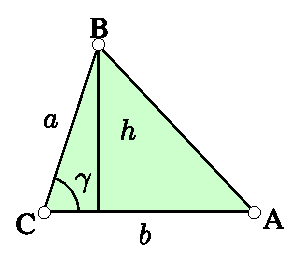
\includegraphics[width=\textwidth]{Triangle_TrigArea.eps}
    \caption{角$C$是锐角}\label{fig:Triangle.TrigArea}
    \end{subfigure}~
    \begin{subfigure}[b]{0.48\textwidth}

    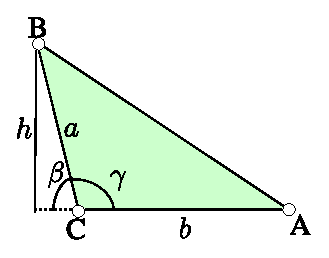
\includegraphics[width=\textwidth]{Triangle_TrigArea2.eps}
    \caption{角$C$是钝角}\label{fig:Triangle.TrigArea2}
    \end{subfigure}
    \end{figure}

如图\ref{fig:Triangle.TrigArea2} 所示,当角$C$是钝角时,$\beta+\gamma=180^{\circ}$。规定$\sin\beta=\sin\gamma$。有$S_{\triangle ABC}=\frac{1}{2}ab\sin\gamma$。

\item 
如图\ref{fig:Cevas_theorem_0} 所示,$O$是三角形$ABC$内部一点,$CO$交$AB$于$F$,$\frac{S_{\triangle ACF}}{S_{\triangle BCF}}=\frac{AF}{BF}=\frac{S_{\triangle AOF}}{S_{\triangle BOF}}$
所以$\frac{AF}{BF}=\frac{S_{\triangle ACO}}{S_{\triangle BCO}}$

    \begin{figure}[!ht]
    \centering
    \begin{subfigure}[b]{0.31\textwidth}
    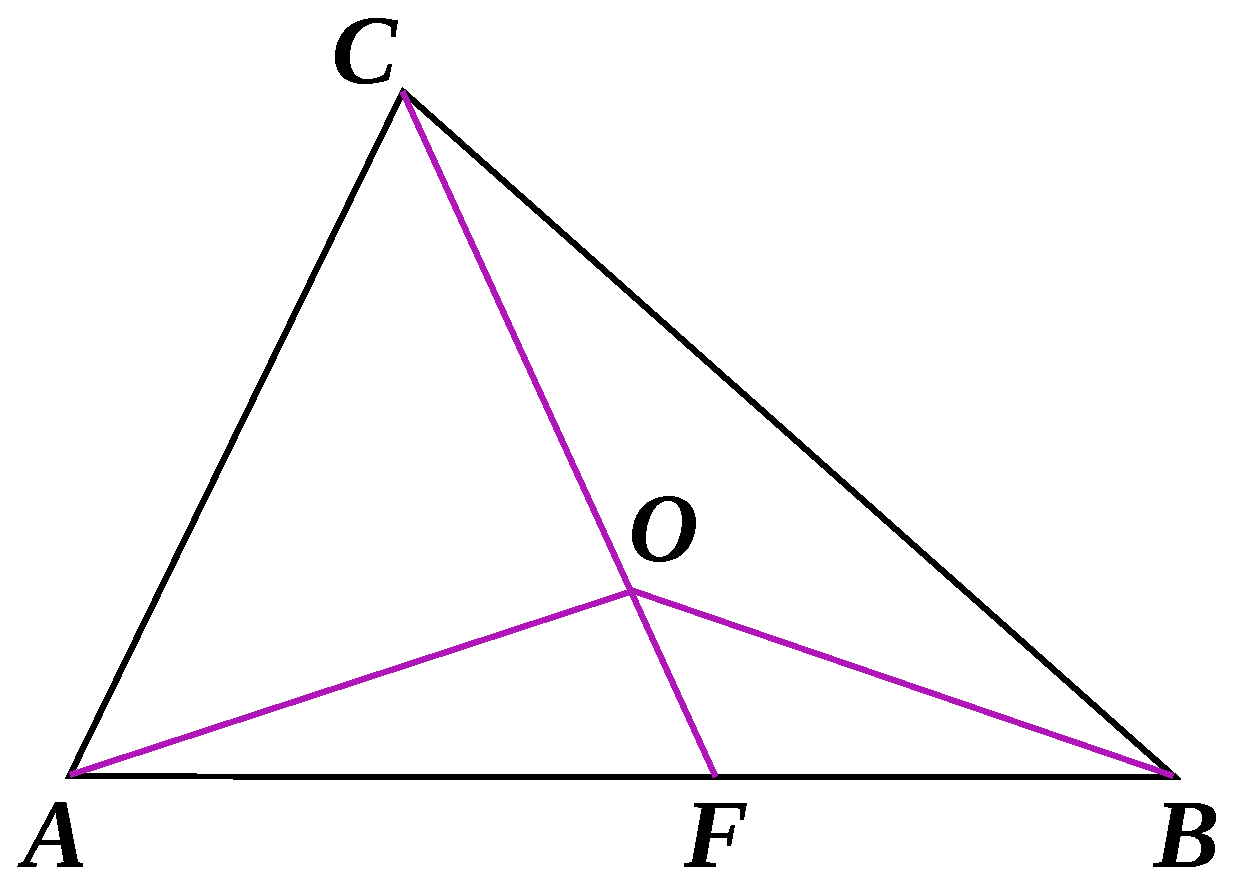
\includegraphics[width=\textwidth]{Cevas_theorem_0.eps}
    \caption{面积比示意图}\label{fig:Cevas_theorem_0}
    \end{subfigure}~
    \begin{subfigure}[b]{0.31\textwidth}

    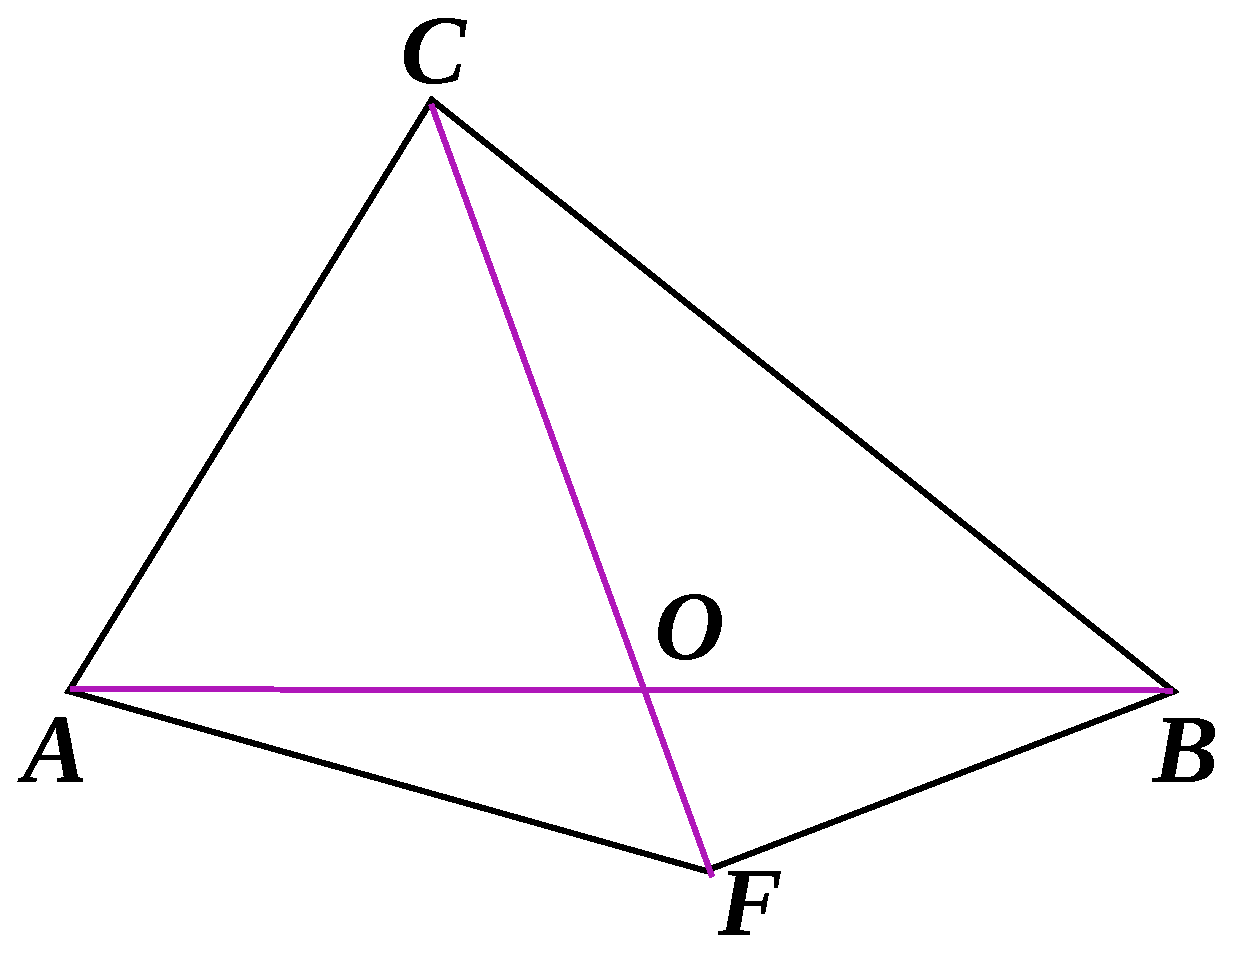
\includegraphics[width=\textwidth]{area_principle.eps}
    \caption{}\label{fig:area_principle}
    \end{subfigure}~
    \begin{subfigure}[b]{0.31\textwidth}
    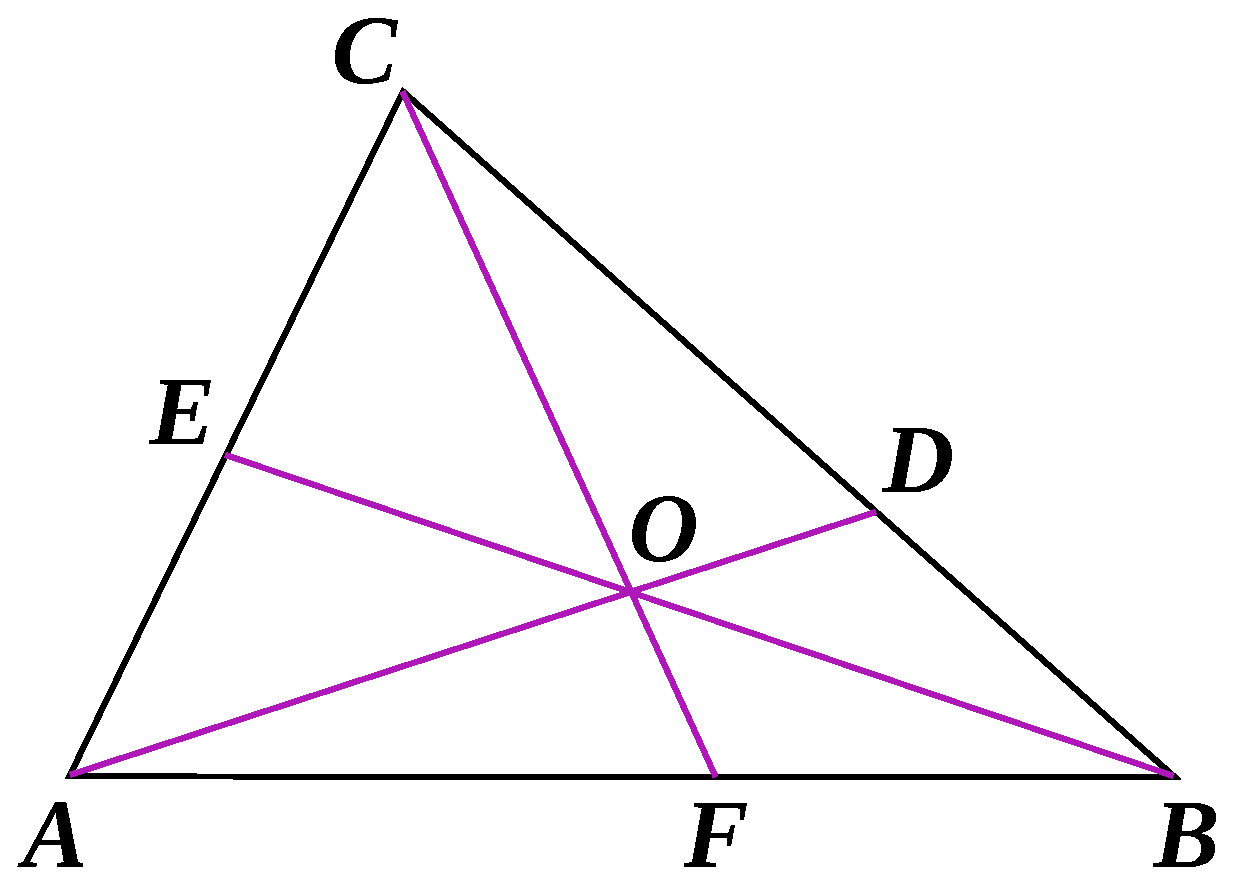
\includegraphics[width=\textwidth]{Cevas_theorem_1.eps}
    \caption{塞瓦定理示意图}\label{fig:Cevas_theorem_1}
    \end{subfigure}
    \end{figure}

如图\ref{fig:area_principle}所示, $\frac{AO}{BO}=\frac{S_{\triangle CAO}}{S_{\triangle CBO}}$
又$\frac{AO}{BO}=\frac{S_{\triangle FAO}}{S_{\triangle FBO}} \Rightarrow\frac{AO}{BO}=\frac{S_{\triangle CAF}}{S_{\triangle CBF}}$


如图\ref{fig:Cevas_theorem_1} 所示,$O$是三角形$ABC$内部一点,$AO,BO,DO$分别交对边于$D,E,F$,则
\begin{equation}\label{eq:Ceva}
\frac{AF}{FB}\cdot\frac{BD}{DC}\cdot\frac{CE}{EA}=1
\end{equation}
\eqref{eq:Ceva}式即为塞瓦定理,(\textbf{作业})试证明该定理。
\item 
课堂练习:
\begin{enumerate}[label=(\roman*)]
\item (面积方法)如图\ref{fig:Acute_Triangle}, 在锐角$\triangle ABC$中,证明
\begin{equation}
\frac{a}{\sin A} = \frac{b}{\sin B} = \frac{c}{\sin C}
\end{equation}
    \begin{figure}[!ht]
    \centering
    \begin{subfigure}[b]{0.4\textwidth}
    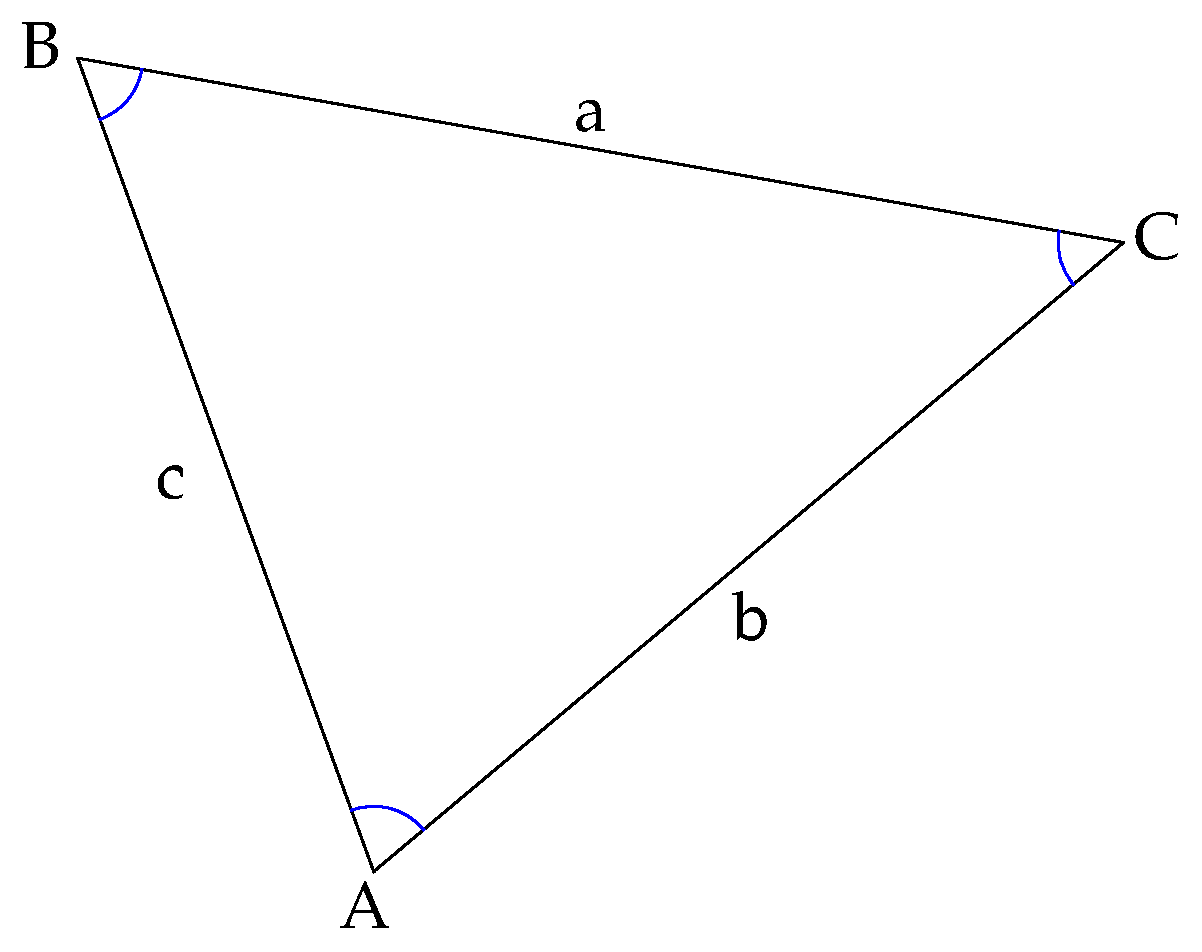
\includegraphics[width=\textwidth]{Acute_Triangle.eps}
    \caption{}\label{fig:Acute_Triangle}
    \end{subfigure}~
    \begin{subfigure}[b]{0.5\textwidth}
    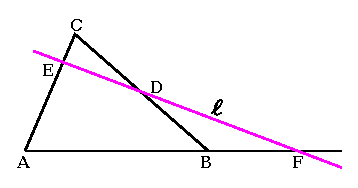
\includegraphics[width=\textwidth]{Menelaus_theorem_1.eps}
    \caption{}\label{fig:Menelaus_theorem_1}
    \end{subfigure}
    \caption{}
    \end{figure}

\item 如图\ref{fig:Menelaus_theorem_1},直线$\ell$交$\triangle ABC$三边或其延长线于$D,E,F$,求证:
\begin{equation}
\frac{AF}{FB}\cdot\frac{BD}{DC}\cdot\frac{CE}{EA}=1
\end{equation}
(提示:利用面积比,$\frac{AF}{FB}=\frac{S_{\triangle ADF}}{S_{\triangle DBF}}$。类似塞瓦定理证明。)

\item 如图 \ref{fig:third_1}, 在等腰$\triangle ABC$中,$CA=CB$,点$P,Q$分别位于线段$AB$的两侧,且$\angle CAP = \angle ABQ,\angle CBP=\angle BAQ$。证明$P,C,Q$三点共线(提示:设$PC$交$AB$于$T$,则$\frac{AT}{TB}=\frac{S_{\triangle PAC}}{S_{\triangle PBC}}=\frac{PA\sin \angle PAC}{PB\angle PBC}$。
设$PQ$交$AB$于$R$,则$\frac{AR}{RB}=\frac{S_{\triangle PAQ}}{S_{\triangle PBQ}}=\frac{PA\cdot AQ}{PB\cdot BQ}=\frac{PA\sin\angle ABQ}{PB\sin\angle BAQ}$
由此推出$\frac{AT}{TB}=\frac{AR}{RB}$)

    \begin{figure}[!ht]
    \centering
    \begin{subfigure}[b]{0.45\textwidth}
    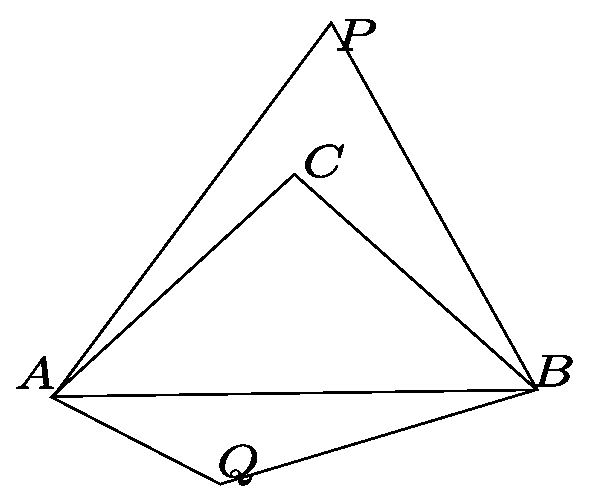
\includegraphics[width=\textwidth]{third_1.eps}
    \caption{}\label{fig:third_1}
    \end{subfigure}~
    \begin{subfigure}[b]{0.45\textwidth}
    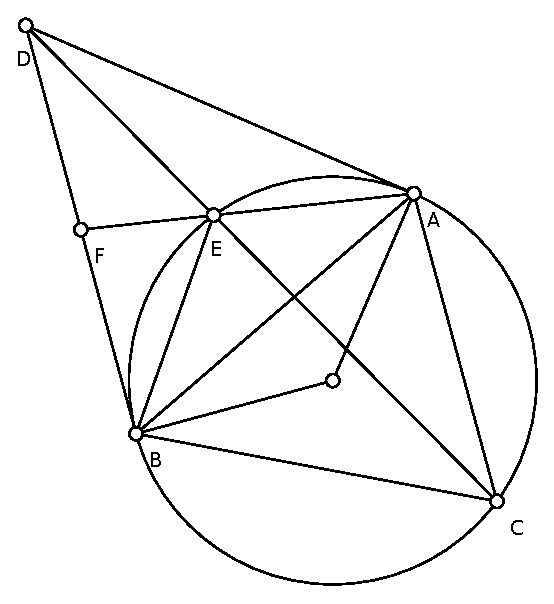
\includegraphics[width=\textwidth]{area.eps}
    \caption{}\label{fig:area}
    \end{subfigure}
    \caption{}
    \end{figure}
\item (\textbf{作业},综合)如图\ref{fig:area},$A,B,C$是圆$\Gamma$上的三点,$AB=BC$。过$A,B$圆$\Gamma$的切线相交于$D$。$DC$交圆$\Gamma$于点$E$,求证$AE$平分线段$BD$。
(提示:证$BD \parallel AC$,
$\frac{DF}{FB}=\frac{DA\sin\angle DAF}{AB\sin \angle EAB}$,$\frac{DA}{AB}=\frac{BD}{BC}=\frac{\sin \angle DCB}{\sin \angle BDC}\Rightarrow$
$
\frac{DF}{FB}=\frac{\sin \angle DCB\cdot \sin\angle DAF}{\sin \angle BDC\cdot \sin \angle EAB}
$。)
\end{enumerate}
\end{enumerate}
\end{document}
